% !TEX root = task-4-6-1.tex
% Editable task bank. Append new BankTask blocks at the end of the document.
\documentclass[12pt,a4paper]{article}
\usepackage{physics-textbook}
\usepackage{graphicx,needspace}
\usetikzlibrary{decorations.pathmorphing}
\newif\ifShowSolutions
\ifdefined\TutorEdition
  \ShowSolutionstrue
\else
  \ShowSolutionsfalse % Change to \ShowSolutionstrue to display solutions.
\fi
\newcounter{banktask}
\newsavebox{\BankTaskBox}
\newcommand{\BankTaskContent}[3]{%
  \noindent\textbf{\thebanktask.}\quad #2\par
  \ifShowSolutions
    \Needspace{50mm}% Keep the solution heading with its opening text or diagram.
    #3\par
    \ifdefined\TutorEdition
      \ifcsname TutorSource#1\endcsname
        \nopagebreak\smallskip{\small\csname TutorSource#1\endcsname\par}%
      \fi
    \fi
  \fi
}
\newcommand{\BankTask}[3]{%
  \refstepcounter{banktask}\par\medskip
  \sbox{\BankTaskBox}{\begin{minipage}{\linewidth}%
    \BankTaskContent{#1}{#2}{#3}\end{minipage}}%
  \ifdim\dimexpr\ht\BankTaskBox+\dp\BankTaskBox\relax>\dimexpr\textheight-20mm\relax
    \Needspace{35mm}\BankTaskContent{#1}{#2}{#3}%
  \else
    \Needspace{\dimexpr\ht\BankTaskBox+\dp\BankTaskBox\relax}%
    \noindent\usebox{\BankTaskBox}\par
  \fi
  \medskip
}
\begin{document}
\BookSubsection{4.6.1}{Собирающая линза: действительное изображение точки}


% Source 97F253: https://ege.fipi.ru/bank/questions.php?search=1&proj=BA1F39653304A5B041B656915DC36B38&qid=97F253
\BankTask{97F253}{
Оптическая сила тонкой собирающей линзы равна \(1\,\text{дптр}\). Точечный источник света, расположенный на главной оптической оси линзы, удалён от неё на три фокусных расстояния. На каком расстоянии от линзы находится изображение источника (в $\text{м}$)?
}{
\smallskip\noindent\textbf{Решение от GPT}\par
Фокусное расстояние \(F=1/D=1\,\text{м}\), расстояние до источника \(a=3F\). По формуле тонкой линзы
\[
\frac1b=\frac1F-\frac1{3F}=\frac2{3F},\qquad b=\frac{3F}{2}=1{,}5\text{ м}.
\]
\(\boxed{1{,}5\text{ м}}\).
}

% Source 50816: https://phys-ege.sdamgia.ru/problem?id=50816
\BankTask{50816}{
\begin{center}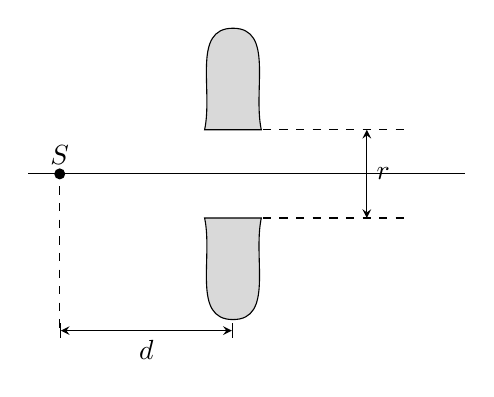
\begin{tikzpicture}[>=stealth]

\draw (-2.6,0)--(2.95,0);\fill (-2.2,0)circle(.07)node[above]{$S$};
\draw[fill=gray!30] (-.36,.56) to[out=78,in=180] (0,1.85) to[out=0,in=102] (.36,.56)--cycle;
\draw[fill=gray!30] (-.36,-.56) to[out=-78,in=180] (0,-1.85) to[out=0,in=-102] (.36,-.56)--cycle;
\draw[dashed](.38,.56)--(2.24,.56) (.38,-.56)--(2.24,-.56);
\draw[<->](1.7,-.56)--(1.7,.56) node[midway,right]{$r$};
\draw[|<->|](-2.2,-1.99)--(0,-1.99)node[midway,below]{$d$};\draw[dashed](-2.2,-.16)--(-2.2,-1.99);
\end{tikzpicture}\end{center}
Точечный источник света находится на главной оптической оси тонкой собирающей линзы. Линзу разрезали на две половины, которые раздвинули на расстояние r  =  $2\,\text{мм}$ (см. рис.). Сделайте рисунок с указанием хода лучей через данную систему. Найдите расстояние от точечного источника света до линзы, если расстояние между действительными изображениями источника l  =  $6\,\text{мм}$. Фокусное расстояние линзы F  =  $40\,\text{см}$.
}{
\smallskip\noindent\textbf{Решение}\par
После того, как линзу разрезали пополам и раздвинули, получилась система из двух линз, у каждой из которой главная оптическая ось поднялась на величину $\frac{r}{2} .$ Построим изображение источника тока через каждую из линз:

\begin{center}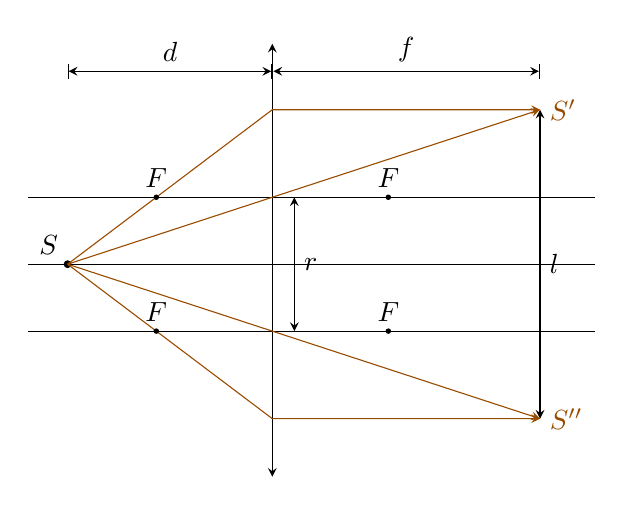
\begin{tikzpicture}[>=stealth]

\draw(-3.1,0)--(4.1,0) (-3.1,.85)--(4.1,.85) (-3.1,-.85)--(4.1,-.85);
\draw[<->](0,-2.7)--(0,2.8);\fill(-2.6,0)circle(.05)node[above left]{$S$};
\draw[orange!60!black,->](-2.6,0)--(0,1.962)--(3.4,1.962)node[right]{$S'$};
\draw[orange!60!black,->](-2.6,0)--(3.4,1.962);
\draw[orange!60!black,->](-2.6,0)--(0,-1.962)--(3.4,-1.962)node[right]{$S''$};
\draw[orange!60!black,->](-2.6,0)--(3.4,-1.962);
\foreach \y in {-.85,.85}{\fill(-1.4733,\y)circle(.035)node[above]{$F$} (1.4733,\y)circle(.035)node[above]{$F$};}
\draw[<->](.28,-.85)--(.28,.85)node[midway,right]{$r$};
\draw[<->](3.4,-1.962)--(3.4,1.962)node[midway,right]{$l$};
\draw[|<->|](-2.6,2.45)--(0,2.45)node[midway,above]{$d$};
\draw[|<->|](0,2.45)--(3.4,2.45)node[midway,above]{$f$};
\end{tikzpicture}\end{center}


\begin{center}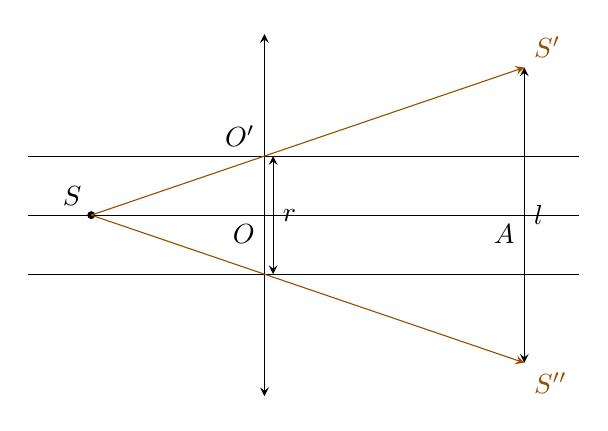
\begin{tikzpicture}[>=stealth]

\draw (-3,0)--(4,0) (-3,.75)--(4,.75) (-3,-.75)--(4,-.75);\draw[<->](0,-2.3)--(0,2.3);
\fill(-2.2,0)circle(.05)node[above left]{$S$};\node[below left]at(0,0){$O$};\node[above left]at(0,.75){$O'$};
\draw[orange!60!black,->](-2.2,0)--(3.3,1.875)node[above right]{$S'$};
\draw[orange!60!black,->](-2.2,0)--(3.3,-1.875)node[below right]{$S''$};
\draw[<->](3.3,-1.875)--(3.3,1.875)node[midway,right]{$l$};\node[below left]at(3.3,0){$A$};
\draw[<->](.11,-.75)--(.11,.75)node[midway,right]{$r$};
\end{tikzpicture}\end{center}


Из подобия треугольников $SOO'$ и $SS'S''$ следует, что $\frac{r}{d} = \frac{l}{d + f} ,$ где f  — расстояние от линзы до изображения. Запишем формулу тонкой собирающей линзы $\frac{1}{d} + \frac{1}{f} = \frac{1}{F} .$ Объединяя формулы, получаем:

\[\frac{1}{d} + \frac{r}{d ( L - r )} = \frac{1}{F} .\]

Выразим расстояние от источника света до линзы:

\[d = \frac{LF}{L - r} = \frac{6 \cdot 40}{6 - 2} = 60 \,\text{см}.\]

Ответ: $60\,\text{см}$.
}

% Source 7902: https://phys-ege.sdamgia.ru/problem?id=7902
\BankTask{7902}{
\begin{center}\begin{tikzpicture}[>=stealth,line width=.65pt]\draw (-4.65,0)--(3.4,0) (-2,-1.95)--(-2,1.95) (0,-1.95)--(0,1.95);\node[above]at(-2,1.95){Э};\node[above]at(0,1.95){Л};\fill (-4.3,.85)circle(.055)node[above left]{$S$};\draw[thin](-4.3,0)--(-4.3,.85)node[midway,left]{$H$};\node[below]at(-3.1,0){$b$};\fill (-2,-.68)circle(.035)node[left]{$A$};\node[right]at(-2,-.36){$h$};\node[above right]at(-2,0){$F$};\fill (2,0)circle(.045)node[above]{$F$};\end{tikzpicture}\end{center}

На расстоянии b = $40\,\text{см}$ от собирающей линзы с фокусным расстоянием $20\,\text{см}$ находится точечный источник света, расположенный на высоте Н = $5\,\text{см}$ от главной оптической оси. В левой фокальной плоскости линзы расположен тонкий экран с малым отверстием  А, находящемся в плоскости рисунка на расстоянии h = $4\,\text{см}$ от главной оптической оси. Изобразите ход луча SA и определите, на каком расстоянии х от плоскости линзы этот луч  от точечного источника, пройдя через отверстие в экране и линзу, пересечет главную оптическую ось. Дифракцией пренебречь.
}{
\smallskip\noindent\textbf{Решение}\par
\begin{center}\begin{tikzpicture}[>=stealth,line width=.65pt]\draw (-4.65,0)--(7,0) (-2,-2.3)--(-2,1.8) (0,-2.3)--(0,1.8);\node[above]at(-2,1.8){Э};\node[above]at(0,1.8){Л};\draw[thin](-4,0)--(-4,.8)node[midway,left]{$H$} (4,0)--(4,-.8)node[midway,above left]{$H\prime$};\draw[blue!70!black] (-4,.8)--(0,.8)--(6.7,-1.88) (-4,.8)--(6.7,-1.34);\draw[green!45!black] (-4,.8)--(0,-2.08)--(7,.16);\draw[->,blue!70!black](-1,.8)--(-.8,.8) (1.1,.36)--(1.3,.28) (.9,-.18)--(1.1,-.22);\draw[->,green!45!black](1.1,-1.728)--(1.3,-1.664);\fill(-4,.8)circle(.045)node[above left]{$S$};\fill(4,-.8)circle(.045)node[below left]{$S\prime$};\fill(-2,-.64)circle(.04)node[below left]{$A$};\node[above right]at(-2,0){$F$};\node[right]at(-2,-.33){$h$};\node[below]at(-3,0){$b$};\fill(2,0)circle(.045)node[above]{$F$};\end{tikzpicture}\end{center}

Построим изображение источника $S',$ используя свойства тонкой линзы: луч, идущий параллельно оптической оси, после преломления в линзе проходит через ее фокус; луч, идущий через середину линзы, не преломляется. Луч SA после преломления в линзе также пройдет через точку $S'$ (см. рис.).
Теперь вычислим, где он пересекает оптическую ось. Луч преломляется в линзе на расстоянии y от оптической оси. Из подобия треугольников находим, что

\[\frac{H + h}{b - F} = \frac{y - h}{F} \Longleftrightarrow y= \frac{F ( H + h )}{b - F} + h= \frac{bh + HF}{b - F} .\]

Из точки А проведем луч через оптический центр линзы О, который не преломляется. Точка А является побочным фокусом линзы, поэтому этот луч параллелен преломленному лучу.
Из подобия треугольников находим, что

$\frac{h}{F} = \frac{y}{x}$
$x=y \cdot \frac{F}{h} = \frac{F}{h} \cdot \frac{bh + HF}{b - F} = \frac{20}{4} \cdot \frac{4 \cdot 40 + 20 \cdot 5}{40 - 20} =65\,\text{см}$

Ответ: ход луча изображен на рисунке, $x=65\,\text{см}.$
}

% Source 26734: https://phys-ege.sdamgia.ru/problem?id=26734
\BankTask{26734}{
Два точечных источника света находятся на главной оптической оси тонкой собирающей линзы на расстоянии L  =  $1\,\text{м}$ друг от друга. Линза находится между ними. Расстояние от линзы до одного из источников x  =  $20\,\text{см}$. Изображения обоих источников получились в одной точке. Найдите оптическую силу линзы. Постройте на отдельных рисунках изображения двух источников в линзе, указав ход лучей.
}{
\smallskip\noindent\textbf{Решение}\par
$1$.  Так как источники находятся с разных сторон от линзы, то для одного из них изображение должно быть действительным, а для другого  — мнимым (см. рис.).
$2$.  Источник, который находится ближе к линзе, дает мнимое изображение.


\begin{center}\begin{tikzpicture}[>=stealth,line width=.65pt]\draw(-4.3,0)--(3.1,0);\draw[<->](0,-2.55)--(0,2.35)node[left]{Л};\draw[orange!80!black] (-3,0)--(2,1.72) (-1.25,0)--(0,1.03)--(2,1.72) (-1.25,-1.03)--(2.25,1.84);\draw[dashed](2,0)--(2,2.18);\fill(-3,0)circle(.045)node[below left]{$S_1^{\prime}$};\fill(-1.25,0)circle(.045)node[below left]{$S_1$};\fill(-2,0)circle(.045)node[below]{$F$};\fill(2,0)circle(.045)node[below]{$F$};\draw[thin](-3,0)--(-3,-2.35) (-1.25,0)--(-1.25,-1.85);\draw[<->](-3,-2.35)--(0,-2.35)node[midway,above]{$f$};\draw[<->](-1.25,-1.8)--(0,-1.8)node[midway,above]{$x$};\draw[->,orange!80!black](1.4,1.515)--(1.7,1.62) (-.75,.412)--(-.5,.618);\end{tikzpicture}\end{center}


 Источник, который находится дальше от линзы, дает действительное изображение.


\begin{center}\begin{tikzpicture}[>=stealth,line width=.65pt]\draw(-3.25,0)--(4,0);\draw[<->](0,-2.55)--(0,2.35)node[left]{Л};\draw[orange!80!black](3.15,0)--(0,1.38)--(-2,0) (3.15,-1.38)--(-2,1);\draw[dashed](-1.25,0)--(-1.25,2.2);\fill(-2,0)circle(.045)node[below left]{$S_2^{\prime}$};\fill(3.15,0)circle(.045)node[below right]{$S_2$};\fill(-1.25,0)circle(.045)node[below]{$F$};\draw[thin](-2,0)--(-2,-2.35) (3.15,0)--(3.15,-2.35);\draw[<->](-2,-2.35)--(0,-2.35)node[midway,above]{$f$};\draw[<->](0,-2.35)--(3.15,-2.35)node[midway,above]{$L-x$};\draw[->,orange!80!black](1.2,.855)--(.9,.986) (-.8,.83)--(-1,.69);\end{tikzpicture}\end{center}


$3$.  Формулы тонкой линзы для двух источников имеют вид:

$\frac{1}{x} - \frac{1}{f} = \frac{1}{F}$ (минус перед f, так как изображение мнимое), ($1$)
$\frac{1}{L - x} + \frac{1}{f} = \frac{1}{F} ,$ ($2$)

 где F  — фокусное расстояние линзы, f  — расстояние от линзы до точки, в которой находятся оба изображения.
$4$.  Решая систему уравнений ($1$)-($2$), получим:

\[F= \frac{2x ( L - x )}{L} .\]

$5$.  Так как оптическая сила линзы $D= \frac{1}{F} ,$ то получим:

\[D= \frac{L}{2x ( L - x )} = \frac{1}{2 \cdot 0{,}2 ( 1 - 0{,}2 )} =3{,}125 \,\text{дптр}.\]

Ответ: D  =  $3{,}125\,\text{дптр}$.
}

% Source 19879: https://phys-ege.sdamgia.ru/problem?id=19879
\BankTask{19879}{
\begin{center}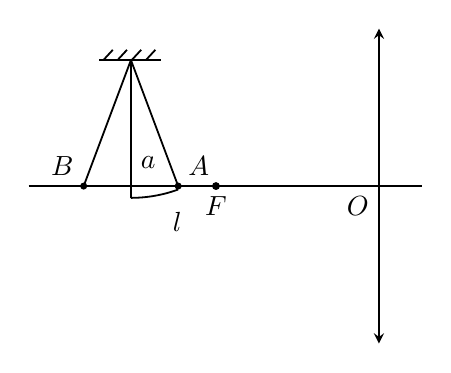
\begin{tikzpicture}[>=stealth,line width=.65pt]\draw(-4,0)--(1,0);\draw[<->](.45,-2)--(.45,2);\draw(-2.7,1.6)--(-3.3,0) (-2.7,1.6)--(-2.1,0) (-2.7,1.6)--(-2.7,-.15);\draw (-2.7,-.15) arc (-90:-70:1.75);\draw(-3.1,1.6)--(-2.32,1.6);\foreach \x in {-3.05,-2.87,...,-2.33} {\draw (\x,1.6)--++(.12,.13);}\fill(-3.3,0)circle(.045)node[above left]{$B$};\fill(-2.1,0)circle(.045)node[above right]{$A$};\fill(-1.62,0)circle(.05)node[below]{$F$};\node[below left]at(.45,0){$O$};\node at(-2.48,.3){$a$};\node at(-2.11,-.45){$l$};\end{tikzpicture}\end{center}

Шарик подвешен на нити и совершает колебания. Его крайние точки, А и B, лежат на оптической оси собирающей линзы силой D  =  $50\,\text{дптр}$. Проекция точки равновесия шарика находится на расстоянии $\sqrt{5}$ см от первого фокуса линзы. Расстояние от нее до крайних точек равно $1\,\text{см}$. Найдите расстояние между изображениями крайних точек A и B в собирающей линзе.
}{
\smallskip\noindent\textbf{Решение}\par
\begin{center}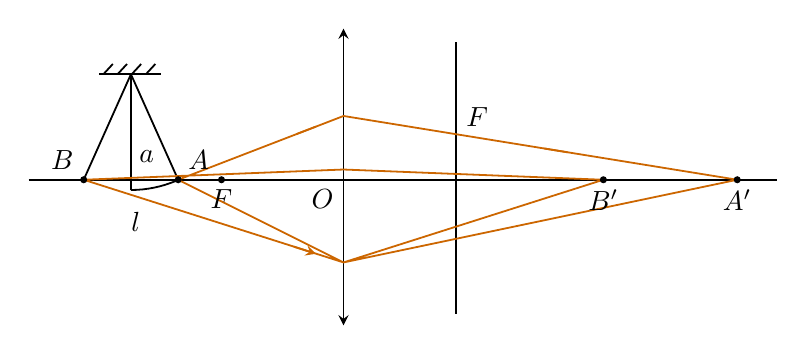
\begin{tikzpicture}[>=stealth,line width=.65pt]\draw(-4,0)--(5.5,0);\draw[<->](0,-1.85)--(0,1.92);\draw(1.43,-1.7)--(1.43,1.75);\draw(-2.7,1.34)--(-3.3,0) (-2.7,1.34)--(-2.1,0) (-2.7,1.34)--(-2.7,-.13);\draw(-2.7,-.13)arc(-90:-67:1.47);\draw(-3.1,1.34)--(-2.32,1.34);\foreach \x in {-3.05,-2.87,...,-2.33} {\draw (\x,1.34)--++(.12,.13);}\draw[orange!80!black](-2.1,0)--(0,.81)--(5,0) (-2.1,0)--(0,-1.05)--(5,0) (-3.3,0)--(0,.13)--(3.3,0) (-3.3,0)--(0,-1.05)--(3.3,0);\draw[->,orange!80!black](-.6,.579)--(-.35,.675) (2.55,.397)--(2.85,.348) (-.63,-.85)--(-.35,-.94);\fill(-3.3,0)circle(.045)node[above left]{$B$};\fill(-2.1,0)circle(.045)node[above right]{$A$};\fill(3.3,0)circle(.045)node[below]{$B^{\prime}$};\fill(5,0)circle(.045)node[below]{$A^{\prime}$};\fill(-1.55,0)circle(.045)node[below]{$F$};\node[above right]at(1.43,.55){$F$};\node[below left]at(0,0){$O$};\node at(-2.5,.3){$a$};\node at(-2.64,-.54){$l$};\end{tikzpicture}\end{center}

Запишем уравнения для тонкой линзы: $\frac{1}{F} = \frac{1}{OB} + \frac{1}{OB'} ;$ $\frac{1}{F} = \frac{1}{OA} + \frac{1}{OA'} .$ По определению $D= \frac{1}{F} ,$ следовательно, $F= \frac{1}{D} =2 \,\text{см}.$ Откуда

$OA=F + l - A=2 + \sqrt{5} - 1=1 + \sqrt{5} \,\text{см},$ 
$OB=F + l + A=3 + \sqrt{5} \,\text{см}.$

Тогда 

$\frac{1}{OB'} = \frac{1}{F} - \frac{1}{OB} =50 - \frac{1}{( 3 + \sqrt{5} ) \cdot 0{,}01} =25 ( \sqrt{5} - 1 ) ;$
$OB'= \frac{1}{25 ( \sqrt{5} - 1 )} = \frac{\sqrt{5} + 1}{100} \,\text{м};$
$\frac{1}{OA'} = \frac{1}{F} - \frac{1}{OA} =50 - \frac{1}{( 1 + \sqrt{5} ) \cdot 0{,}01} =25 ( 3 - \sqrt{5} ) ;$
$OA'= \frac{1}{25 ( 3 - \sqrt{5} )} = \frac{3 + \sqrt{5}}{100} \,\text{м};$
$|OA' - OB'|=| \frac{\sqrt{5} + 1 - 3 - \sqrt{5}}{100} |= \frac{1}{50} \,\text{м} = 2\,\text{см}.$

Ответ: $|OA' - OB'|=2\,\text{см}.$
}

\end{document}
